% !TEX TS-program = pdflatex
% !TEX encoding = UTF-8 Unicode

% This is a simple template for a LaTeX document using the "article" class.
% See "book", "report", "letter" for other types of document.

\documentclass[11pt]{article} % use larger type; default would be 10pt
\usepackage[utf8]{inputenc}
% === MY PACKAGES ===
\usepackage{amssymb}
\usepackage{amsmath}
\usepackage{bm}
%\newcommand{\cc}{\boldsymbol{\sigma}} % Ican't find corresponding package
\newcommand{\cc}{\bm{\sigma}}
% === ===

\usepackage{geometry} % to change the page dimensions
\geometry{a4paper} % or letterpaper (US) or a5paper or....
% \geometry{margin=2in} % for example, change the margins to 2 inches all round
% \geometry{landscape} % set up the page for landscape
\usepackage{graphicx} % support the \includegraphics command and options
% \usepackage[parfill]{parskip} % Activate to begin paragraphs with an empty line rather than an indent
\usepackage{booktabs} % for much better looking tables
\usepackage{array} % for better arrays (eg matrices) in maths
\usepackage{paralist} % very flexible & customisable lists (eg. enumerate/itemize, etc.)
\usepackage{verbatim} % adds environment for commenting out blocks of text & for better verbatim
\usepackage{subfig} % make it possible to include more than one captioned figure/table in a single float
\usepackage{fancyhdr} % This should be set AFTER setting up the page geometry
\pagestyle{fancy} % options: empty , plain , fancy
\renewcommand{\headrulewidth}{0pt} % customise the layout...
\lhead{}\chead{}\rhead{}
\lfoot{}\cfoot{\thepage}\rfoot{}
\usepackage{sectsty}
\allsectionsfont{\sffamily\mdseries\upshape} % (See the fntguide.pdf for font help)
\usepackage[nottoc,notlof,notlot]{tocbibind} % Put the bibliography in the ToC
\usepackage[titles,subfigure]{tocloft} % Alter the style of the Table of Contents
\renewcommand{\cftsecfont}{\rmfamily\mdseries\upshape}
\renewcommand{\cftsecpagefont}{\rmfamily\mdseries\upshape} % No bold!

%%% The "real" document content comes below...

\title{Table of results}
\author{Fipipp Uskov}
%\date{} % Activate to display a given date or no date (if empty),
         % otherwise the current date is printed 


\begin{document}
\maketitle

\section{Results}

$$ H=J\sum_{<i,j>}(\cc_i\cc_j) = 2J\sum_{<i,j>}(\bm{s}_i\bm{s}_j) $$

$$ E_{gs\;full}/N\geqslant $$

\subsection{1d case}

\begin{tabular}{|l|l|l|}
\hline
cluster & Shredinger & Variational \\
\hline

\includegraphics[width=0.3\textwidth]{line4.png} & -2.1547 & -2.09548 \\
\hline

\includegraphics[width=0.3\textwidth]{line5.png} & -1.92789 & -1.91063 \\
\hline

\includegraphics[width=0.3\textwidth]{line6.png} & -1.99486 & -1.94983 \\
\hline

\includegraphics[width=0.3\textwidth]{line7.png} & -1.89083 & -1.87265 \\
\hline

\includegraphics[width=0.3\textwidth]{line8.png} & -1.92853 & -1.8388 \\
\hline
\end{tabular}

\subsection{2d case}

\begin{tabular}{|l|l|l|}
\hline
cluster & Shredinger & Variational \\
\hline
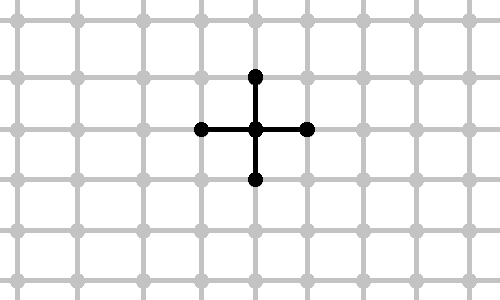
\includegraphics[width=0.3\textwidth]{lattice-crest.png} & -3 & -3 \\
\hline
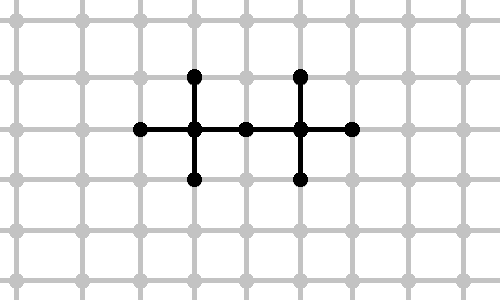
\includegraphics[width=0.3\textwidth]{lattice-double-crest.png} & -2,9685 & -2.9657 \\
\hline
\end{tabular}

\section{Basis overflow hypotesis}

All linear dependencies in basis (because of which basis is overcrowded) are derived from equation (1) and (3).
But $(1,2)\;\Rightarrow\;(3)$.
It was checked up to 10 spins.

$$+(\cc_1\cc_2)(\cc_3\cc_4\cc_5)-(\cc_1\cc_3)(\cc_2\cc_4\cc_5)+(\cc_1\cc_4)(\cc_2\cc_3\cc_5)-(\cc_1\cc_5)(\cc_2\cc_3\cc_4)=0   \qquad(1)$$
$$(\cc_1\cc_2\cc_3)(\cc_4\cc_5\cc_6) = \mathrm{det}
\begin{pmatrix}
(\cc_1\cc_4) & (\cc_2\cc_4) & (\cc_3\cc_4) \\
(\cc_1\cc_5) & (\cc_2\cc_5) & (\cc_3\cc_5) \\
(\cc_1\cc_6) & (\cc_2\cc_6) & (\cc_3\cc_6) \\
\end{pmatrix}
\qquad(2)
$$
$$(1,2)\;\Rightarrow\quad
\mathrm{det}
\begin{pmatrix}
(\cc_1\cc_5) & (\cc_2\cc_5) & (\cc_3\cc_5) & (\cc_4\cc_5) \\
(\cc_1\cc_6) & (\cc_2\cc_6) & (\cc_3\cc_6) & (\cc_4\cc_6) \\
(\cc_1\cc_7) & (\cc_2\cc_7) & (\cc_3\cc_7) & (\cc_4\cc_7) \\
(\cc_1\cc_8) & (\cc_2\cc_8) & (\cc_3\cc_8) & (\cc_4\cc_8) \\
\end{pmatrix} =0
\qquad(3)
$$


\[\begin{array}{l}
{\rm{ + (}}{{\bf{\sigma }}_1}{{\bf{\sigma }}_2}{\rm{)(}}{{\bf{\sigma }}_3}{{\bf{\sigma }}_4}{{\bf{\sigma }}_5}{\rm{) - (}}{{\bf{\sigma }}_1}{{\bf{\sigma }}_3}{\rm{)(}}{{\bf{\sigma }}_2}{{\bf{\sigma }}_4}{{\bf{\sigma }}_5}{\rm{)}} + {\rm{(}}{{\bf{\sigma }}_1}{{\bf{\sigma }}_4}{\rm{)(}}{{\bf{\sigma }}_2}{{\bf{\sigma }}_3}{{\bf{\sigma }}_5}{\rm{) - (}}{{\bf{\sigma }}_1}{{\bf{\sigma }}_5}{\rm{)(}}{{\bf{\sigma }}_2}{{\bf{\sigma }}_3}{{\bf{\sigma }}_4}{\rm{)}} = 0\qquad (1)\\

\qquad \qquad {\rm{(}}{{\bf{\sigma }}_1}{{\bf{\sigma }}_2}{{\bf{\sigma }}_3}{\rm{)(}}{{\bf{\sigma }}_4}{{\bf{\sigma }}_5}{{\bf{\sigma }}_6}{\rm{) = }}\det \left( {\begin{array}{*{20}{c}}
{{\rm{(}}{{\bf{\sigma }}_1}{{\bf{\sigma }}_4}{\rm{)}}}&{{\rm{(}}{{\bf{\sigma }}_2}{{\bf{\sigma }}_4}{\rm{)}}}&{{\rm{(}}{{\bf{\sigma }}_3}{{\bf{\sigma }}_4}{\rm{)}}}\\
{{\rm{(}}{{\bf{\sigma }}_1}{{\bf{\sigma }}_5}{\rm{)}}}&{{\rm{(}}{{\bf{\sigma }}_2}{{\bf{\sigma }}_5}{\rm{)}}}&{{\rm{(}}{{\bf{\sigma }}_3}{{\bf{\sigma }}_5}{\rm{)}}}\\
{{\rm{(}}{{\bf{\sigma }}_1}{{\bf{\sigma }}_6}{\rm{)}}}&{{\rm{(}}{{\bf{\sigma }}_2}{{\bf{\sigma }}_6}{\rm{)}}}&{{\rm{(}}{{\bf{\sigma }}_3}{{\bf{\sigma }}_6}{\rm{)}}}
\end{array}} \right)\qquad (2)\\

\qquad \qquad (1,2) \Rightarrow \;\;\;\det \left( {\begin{array}{*{20}{c}}
{{\rm{(}}{{\bf{\sigma }}_1}{{\bf{\sigma }}_5}{\rm{)}}}&{{\rm{(}}{{\bf{\sigma }}_2}{{\bf{\sigma }}_5}{\rm{)}}}&{{\rm{(}}{{\bf{\sigma }}_3}{{\bf{\sigma }}_5}{\rm{)}}}&{{\rm{(}}{{\bf{\sigma }}_4}{{\bf{\sigma }}_5}{\rm{)}}}\\
{{\rm{(}}{{\bf{\sigma }}_1}{{\bf{\sigma }}_6}{\rm{)}}}&{{\rm{(}}{{\bf{\sigma }}_2}{{\bf{\sigma }}_6}{\rm{)}}}&{{\rm{(}}{{\bf{\sigma }}_3}{{\bf{\sigma }}_6}{\rm{)}}}&{{\rm{(}}{{\bf{\sigma }}_4}{{\bf{\sigma }}_6}{\rm{)}}}\\
{{\rm{(}}{{\bf{\sigma }}_1}{{\bf{\sigma }}_7}{\rm{)}}}&{{\rm{(}}{{\bf{\sigma }}_2}{{\bf{\sigma }}_7}{\rm{)}}}&{{\rm{(}}{{\bf{\sigma }}_3}{{\bf{\sigma }}_7}{\rm{)}}}&{{\rm{(}}{{\bf{\sigma }}_4}{{\bf{\sigma }}_7}{\rm{)}}}\\
{{\rm{(}}{{\bf{\sigma }}_1}{{\bf{\sigma }}_8}{\rm{)}}}&{{\rm{(}}{{\bf{\sigma }}_2}{{\bf{\sigma }}_8}{\rm{)}}}&{{\rm{(}}{{\bf{\sigma }}_3}{{\bf{\sigma }}_8}{\rm{)}}}&{{\rm{(}}{{\bf{\sigma }}_4}{{\bf{\sigma }}_8}{\rm{)}}}
\end{array}} \right) = 0
\end{array}\]

\end{document}
